\documentclass[10pt]{article} 
\usepackage[final]{graphicx} 
\usepackage{amsfonts} 
 \usepackage{amsmath}
\usepackage{tikz, flowchart}
\usetikzlibrary{arrows}
\topmargin-.5in 
\textwidth6.6in 
\textheight9in 
\oddsidemargin0in 
 
\def\ds{\displaystyle} 
\def\d{\partial} 

 
\begin{document} 


\centerline{\large \bf Wine, Ebola and Terrorism}

\vspace{.1truein}

\def\thefootnote{\arabic{footnote}}
\begin{center}
  Hsuan-Wei Lee\footnote{Department of Mathematics, UNC Chapel Hill},
  Anzhelika Lyubenko\footnote{Department of Mathematical and Statistical Sciences, University of Colorado Denver},
  Yuhang Ma\footnote{Department of Operations Research and Information Engineering, Cornell University},
  Emily Meissen\footnote{Department of Applied Mathematics, University of Arizona},
  Daniela Velez-Rendon\footnote{Department of Bio-engineering, University of Illinois at Chicago},
    Nara Yoon\footnote{
Department of Mathematics, Applied Mathematics and Statistics, Case Western Reserve University}
\end{center}

%\vspace{.1truein}

\begin{center}
Faculty Mentors: John Peach \footnote{MIT Lincoln Labs}, Cammey Cole Manning\footnote{Meredith College},
Christian Gunning\footnote{NCSU}
\end{center}


\vspace{.3truein}
\centerline{\bf Abstract}

\begin{itemize}
\item Summarize the results presented in the report, and the contributions
of your research.

\item Readers should not have to look at the rest of the paper in order to 
understand the abstract.

\item Keep it short and to the point.
\end{itemize}
%
%
%
%
% INTRODUCTION
%
%
%
%
%
\section{Introduction}
Bacteria growth during wine making, spread of infectious diseases and recruitment to extremists organizations can be modeled in a similar way - either by exponential or logistic growth models. For the purposes of this paper we focus solely on modeling the spread of Ebola through the West African region that contains Guinea, Sierra Leone, Liberia and Nigeria throughout 2014 - 2015 outbreak. \\
%
%
%
Ebola was first discovered in 1976. Since then, there were a few minor cases as well as a few outbreaks reported by the Center for Disease Control and Prevention. However, until 2014 all outbreaks had a reported number of deaths that did not exceed 500. The outbreak of 2014 is considered different. It already took thousands of lives and received an extensive media coverage over the past 2 years.
%
%
%
It has been reasoned that the current outbreak is different because it was the first time Ebola was contracted in the West Africa as opposed to Central Africa where it was first discovered. Early symptoms are flu-like: fever, headache, fatigue and joint pain. Diseases like HIV and Malaria, which are common to the region, have the same symptoms. As Ebola progresses, the infected experiences abdominal pain, diarrhea, vomiting and rashes. The virus is contracted through direct contact with bodily fluids and secretion: blood, saliva, urine, fecal matter. Once virus is contracted, the incubation period may last up to 2 weeks making intervention measures like tracking difficult. 
%
%
%
\\A variety of cultural and economic factors have contributed to the spread of the disease: lack of medical centers in some regions and poor sensitization practices in such centers, distrust in the western medicine, poverty, traditional burial ceremony which includes physical contact with the diseased. \\
%
%
%
Traditionally, infectious diseases are modeled by an SIR model with possible modifications. In the case of Ebola, Lekone and Finkenstäd \cite{Lekone2006} consider a four compartment model, inserting an "Exposed" state between "Susceptible" and "Infected". A variety of authors present a five-compartment model \textbf{what do they include}. Examples of such papers are \textbf{BLAH! CITE}. A six-compartment model, presented by Legrand \cite{Legrand2007} and Rivers\cite{Rivers2014} differentiates between the modes of transition of the disease, i.e. a virus can be transmitted in the community, at hospitals and medical centers or at funerals. Agent-based models include Siettos et al \cite{Siettos2015} and Merler et al\cite{Merler2015}. A variety of models examine the effectiveness of intervention measures: contact tracing by Webb et al \cite{Webb2015}, travel restrictions by Poletto et al \cite{Poletto2014},     Rivers et al did something else \cite{Rivers2014}\\\\
Somewhere later: We used InsightMaker platform to build our model and simulate stepping forward through time. More details about the platform and its functionality can be found in Fortmann-Roe's review \cite{FortmannRoe}. The platform uses fourth order Runge-Kutta differential equation solver for the system dynamics model and  first order Euler approximation for the Agent-Based model.
\\\\

It should be written as much as possible in non-technical terms, so that a
lay reader can understand the context and the contribution of the paper.

\begin{itemize}
\item Describe the problem you are trying to solve, the approach
you took, and summarize your contribution and results.

\item Review the history of this problem, and existing literature.

\item Give an outline of the rest of the paper.
\end{itemize}

The rest of the paper is organized as follows. In section 2 we present technical description of the problem. Section 3 describes our mathematical model. Section 4 presents the results of numerical experiments. Section 5 concludes.

\section{The Problem}
\begin{itemize}
\item Give a precise technical description of your problem. 

\item State and justify all your assumptions. 

\item Define notation. 

\item Describe your data, how you collected them, their properties,
and whether you did 
anything to them (removed noise, filled in missing data, 
applied normalizations).
\end{itemize}

\section{The Approach}

\subsection{Strategy}
In order to propose a more accurate model and compare the results among different programming  languages, the compartment flow model of the Ebola Epidemic in West Africa, 2014, was modeled with a System Dynamics (SD) and Agent Based Model (ABM) approaches.  Insight Maker and Mathematica was utilized  for the SD, and Insight Maker and Python for the ABM.

\subsection{Assumptions}
\begin{itemize}
\item For the present study, it was considered information of two countries that experienced the Ebola Outbreak, Liberia and Sierra Leone.
\item Time frame: It was divided into stages, first, beginning from the Ebola Outbreak in March 2014 to the International Intervention in September 2014, and second, from the International Intervention to the present.
\item It was ignored all the possible births and natural deaths ocurred during the chosen timelime, because our simulation is for short period of time, our model was considered as a closed system.
\end{itemize}

\subsection{Factors Considered}
\begin{itemize}
\item Transmission method.
\item Probability of transfer.
\item Population size/density.
\item Amount of travel (length of time, destinations, mode of travel, local travel).
\item Connectedness.
\item Length of time Ebola virus remains in deceased.
\item Rate of recovery.
\item Rate of death.
\item Rate of diagnosis and accuracy.
\item Rate of hospitalization.
\item Hospital capacity.
\item Wealth of the region, local government involment.
\item Interaction with infected animals.
\item Household size.
\item "Belief" rate.
\item Cleanliness.
\item International help.
\item Following protocols.
\item Access to healthcare, lack of ambulances.
\item Cummunity/hospital/burial have different transfer rates.
\end{itemize}

\subsection{Software}
\begin{itemize}
\item Insight Maker: SD and ABM
\item Mathematica: SD
\item Python: ABM

\end{itemize}
\section{Data}
The United Nation reports that the last Census for the countries of Guinea, Sierra Leone, Liberia and Nigeria  was conducted in 2014, 2004, 2008 and 2006 respectively. Due to the need for estimating more current demographic data, we used CIA Factbook estimates. 

\section{Computational Experiments}

\subsection{Compartment Model: System Dynamics}
Based on the compartmental model and parameters published by Rivers et al. in October 2014, it was modeled a similar approach in Insight Maker.  This particular model, divides the population into six different compartments; the Susceptible persons (S) could turn into Exposed (E), if they were in contact with an infections individual, initiating a trantition to the Infectious (I) state after the incubation period of the disease, subsequently, acquiring the capacity of infecting others. A percentage of the I class individuals may be Hospitalized (H). There are two possible outcomes for the untreated individuals in I and the treated patients in H, individuals may die, with a probability of infecting other people during the resultant Funeral (F), before the virus is removed from the individual (R), or the patients may recover, at this stage, it can be cosidered equivalently removed. Figure  \ref{fig:compartment} depicts the implemented compartment model. \\

\begin{figure}
  \centering
  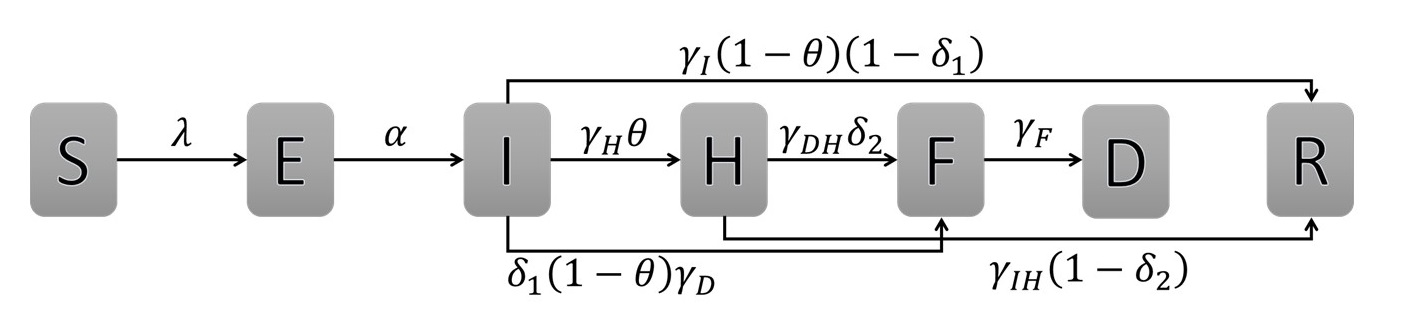
\includegraphics[width=0.7\textwidth]{compartment}
  \caption{\bf Compartment Model of the Ebola Epidemic in Liberia and Sierra Leone \newline  Being S: Susceptible, E: Exposed, I: Infectious, H: Hospitalized, F: Funeral and R: Removed/Recovered. All the possible flows are specified by the arrows and the parameters that direct them. Note that $\lambda = \beta_{I}I+\beta_{H}H+\beta_{F}F $, being a combination of all the $\beta$ transmission terms shown in Table \ref{tab:parameters}} 
\label{fig:compartment} 
\end{figure}

 

 The governing equations of the system described above are the following: \\

\begin{eqnarray} 
\frac{dS}{dt} = - \frac{\beta_{I}SI+\beta_{H}SH+\beta_{F}SF}{N}\\
\frac{dE}{dt} =  \frac{\beta_{I}SI+\beta_{H}SH+\beta_{F}SF}{N}-\alpha E\\
\frac{dI}{dt} =  \alpha E - [\gamma_{H}\theta + \gamma_{I}(1-\theta)(1-\delta_{1})+\gamma_{D}(1-\theta)\delta_{1}]I\\
\frac{dH}{dt} = \gamma_{H}\theta I - [\gamma_{DH}\delta_{2}+\gamma_{IH}(1-\delta_{2})]H\\
\frac{dF}{dt} = \gamma_{D}(1-\theta) \delta_{1} I + \gamma_{DH}\delta_{2} H-\gamma_{F} F\\
\frac{dR}{dt} = \gamma_{I}(1-\theta)(1- \delta_{1}) I + \gamma_{IH}(1-\delta_{2}) H-\gamma_{F} F
\end{eqnarray}\\

where each of the parameters are defined on Table \ref{tab:parameters} \\

\begin{table}[ht]
\caption{Model Parameters for Ebola Epidemic in Liberia and Sierra Leone Before the International Intervention (September 2014)} % title of Table
\centering % used for centering table
\begin{tabular}{c c c } 
\hline\hline %inserts double horizontal lines
Parameter & Liberia & Sierra Leone \\ [0.5ex] % inserts table
%heading
\hline % inserts single horizontal line
Contact Rate, Community  ($\beta_{I}$) & 0.160 & 0.128  \\ 
Contact Rate, Hospital  ($\beta_{H}$) & 0.062 & 0.080  \\
Contact Rate, Funeral  ($\beta_{F}$) & 0.489 & 0.111 \\
Incubation Period (${1}/{\alpha}$) & 12 days & 10 days  \\
Time until Hospitalization (${1}/{\gamma_{H}}$) & 3.24 days & 4.12 days  \\
Time froml Hospitalization to Death (${1}/{\gamma_{DH}}$) & 10.07 days & 6.26 days  \\ 
Duration of Traditional Funeral (${1}/{\gamma_{F}}$) & 2.01 days & 4.50 days  \\
Duration of Infection (${1}/{\gamma_{I}}$) & 15.00 days & 20.00 days  \\
Time from Infection to Death (${1}/{\gamma_{D}}$) & 13.31 days & 10.38 days  \\
Time from Hospitalization to Recovery (${1}/{\gamma_{IH}}$) & 15.88 days & 15.88 days  \\
Probablity a Case is Hospitalized ($\theta$) & 0.197 & 0.197  \\
Case Fatality Rate, Unhospitalized ($\delta_{1}$) & 0.500 & 0.750  \\
Case Fatality Rate, Hospitalized ($\delta_{2}$) & 0.500 & 0.750  \\ [1ex] 
\hline 
\end{tabular}
\label{tab:parameters}
\end{table}

\subsection{Compartment Model: Agent Dynamics}
The agent-based model created in Insight Maker also used the data from Rivers et al. with the same states and parameter names as the System Dynamics model. The transitions between the states are described as:\\

\begin{table}[ht]
\begin{center}
\begin{tabular}{c | l | l}
{\bf Transition} & {\bf Type } & {\bf Value}\\\hline
$S\rightarrow E$ & Probability & $\min(1,\xi_5\beta_{fam}+\xi_{100}\beta_{com}+\xi_{10}\beta_F)$\\
$E\rightarrow I$ & Timeout & $1/\alpha$\\
$I\rightarrow H$ & Probability & $\theta\gamma_H$\\
$I\rightarrow F$ & Probability & $(1-\theta)\delta_1\gamma_D$\\
$I\rightarrow R$ & Probability & $(1-\theta)(1-\delta_{1})\gamma_I$\\
$F\rightarrow R$ & Timeout & ${1}/{\gamma_{F}}$\\
$H\rightarrow R$ & Timeout & $\delta_{2}/{\gamma_{DH}} + (1-\delta_{2})/{\gamma_{IH}}$\\
\end{tabular}
\end{center}
\end{table}
\noindent where $\xi_{i}$ is the number of infected people within the individual's $i$ closest neighbors, $\beta_{fam}$ is the family contact rate, and $\beta_{com}$ is the community contact rate (maybe same?). The probability of contracting Ebola depends on the number of infected people within the individual's family or neighbors, and funerals are assumed to be attended by the deceased's 10 nearest neighbors.

\begin{figure}
\caption{The agent-based Insight Maker model.}
\end{figure}

\begin{figure}
\caption{A simulation of the agent-based Insight Maker model with $\beta_{fam}=0.4$ and $\beta_{com}=0.01$.}
\end{figure}

\subsubsection{Insight Maker}
bdv

\subsubsection{Mathematica}
vxzv

\subsection{Compartment Model: Agent Based Model}
The next model we consider is an agent-based model. Each individual in the population can be in either of 7 states discussed above: susceptible, exposed, infected, hospitalized, funeral, recovered or dead. The flow between two states is a  probability of transition from one state to another for a typical individual. We represent our model in Figure~\ref{ABM}. In each time step individuals who are susceptible to contracting a virus can either transition to exposed state with probability $p_{SE}$ or stay susceptible with probability $1-p_{SE}$. An individuals in the exposed state transitions to infected with probability $p_{EI}$ and stays exposed with probability $1-p_{EI}$. An individual who is infected can stay infected, recover, go to a hospital or die and transition to funeral state with probabilities $p_{II},\, p_{IR},\, p_{IH}$ and $p_{IF}$ respectively. Recovery is considered a terminal state so individuals in this state remain in it for the remaining duration of the simulation. Hospitalized individuals may stay hospitalized, transition to recovered or funeral with probabilities $p_{HH}, \, p_{HR}$ and $p_{HF}$.   We assume that the individual who dies from Ebola remains infectious through the duration of the entire burial ceremony and no precautions are taken against disease transmission. Safely buried individuals are considered dead and noninfectious and remain in this state for the remaining time of the simulation.  Probability of transition for each state are as follows: \\\\
For duration of the simulation we ignore deaths of other causer and focus only on those individuals who died due to Ebola virus. We assume that every individual who dies has a funeral.
\begin{itemize}
 \item g
\end{itemize}
%  \begin{tikzpicture}[node distance=2cm, font=\tiny]
%        \node [draw, terminal]  (start) at (0,0) {Start};
%        \node [draw, predproc, right of= start] (acquire)(write) {Acquire Image};
%
%%% paths
%    \draw[->](work) -- node[above]{yes}(end);
%    \end{tikzpicture}
\begin{figure}[h!]
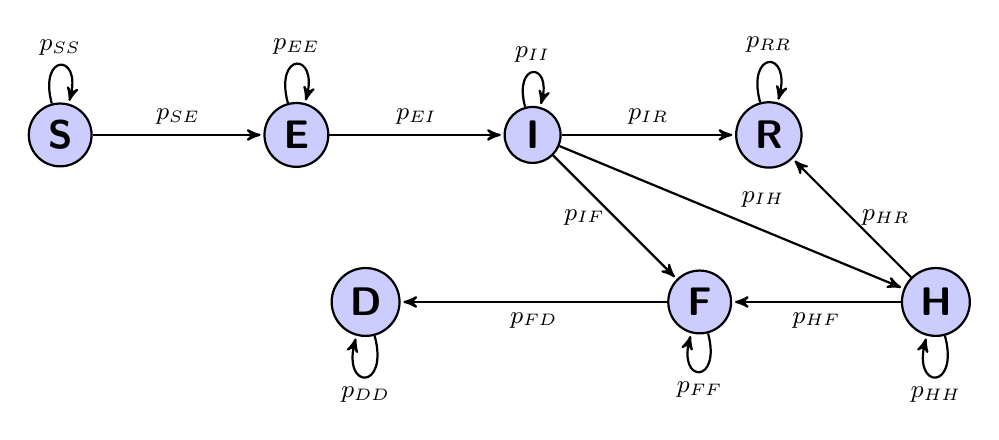
\begin{tikzpicture}[->,>=stealth',shorten >=1pt,auto,node distance=3cm,
  thick,main node/.style={circle,fill=blue!20,draw,font=\sffamily\Large\bfseries}]

  \node[main node] (1) {S};
  \node[main node] (2) [right of=1] {E};
  \node[main node] (3) [right of=2] {I};
  \node[main node] (4) [right of=3] {R};
    \node[main node] (5) [below left of=3] {D};
      \node[main node] (6) [below right of=3] {F};
        \node[main node] (7) [right of=6] {H};

  \path[every node/.style={font=\sffamily\small}]
    (1) %edge node [left] {0.6} (4)
        edge node {$p_{SE}$} (2)
        edge [loop above] node {$p_{SS}$} (1)
    (2) %edge node [right] {0.4} (1)
        edge node {$p_{EI}$} (3)
         edge [loop above] node {$p_{EE}$} (2)
        %edge [loop left] node {0.4} (2)
       % edge [bend right] node[left] {0.1} (3)
    (3) %edge node [right] {0.8} (2)
       % edge [bend right] node[right] {0.2} (4)
       edge node {$p_{IR}$} (4)
       edge node[left] {$p_{IF}$} (6)
       edge node {$p_{IH}$} (7)
        edge [loop above] node {$p_{II}$} (3)
    (4)% edge node [left] {0.2} (3)
        %edge [loop right] node {0.6} (4)
        %edge [bend left] node[right] {0.2} (1);
         edge [loop above] node {$p_{RR}$} (4)
       
(6) edge node{$p_{FD}$} (5) 
edge [loop below] node {$p_{FF}$} (6)     
(7) edge node[right]{$p_{HR}$} (4) 
edge [loop below] node {$p_{HH}$} (7)
  (7) edge node{$p_{HF}$} (6)      
 (5) edge [loop below] node {$p_{DD}$} (5)
        ;
        
\end{tikzpicture}
\caption{Spread of the disease: Agent-based model. Each node represents an individual's state; each link is a possible transition}
\label{ABM}
\end{figure}

\begin{align*}
&t_{IP}\, \text{be the incubation period, i.e. time during which the individual has the virus in his body but does not yet show severe symptoms}\\
&t_{ID} \,\text{infection duration time ater the onset of severe symptoms}\\
&t_{H} \, \text{time to hospitalization after manifistation of severe symptoms}\\
& t_{IF} \, \text{time from the onset of severe symptoms to funeral}\\
& t_{HF} \, \text{time from patient's arrival at the hospital to fueral}\\
& t_{HR} \, \text{time from patient's arrival at the hospital to recovery}\\
& t_{DF} \, \text{duration of traditional funeral}
\end{align*}


\begin{subequations}
\begin{alignat}{1}
&p_{SE}=\beta_I\cdot I/N+\beta_H\cdot H/N+\beta_F\cdot F/N\\
&p_{SS}=1-p_{SE}\\
&p_{EE}=1-\frac{1}{t_{IP}}\\
&p_{EI}=\frac{1}{t_{IP}}\\
&p_{II}=\frac{1}{t_{ID}}\\
&p_{IH}=\frac{1}{t_{H}}\\
&p_{IF}= \frac{1}{t_{IF}}\\
&p_{IR}=1-p_{II}-p_{IH}-p_{IF}\\
&p_{HF}=\frac{1}{t_{HF}}\\
&p_{HR}=\frac{1}{t_{HR}}\\
&p_{HH}=1-p_{HF}-p_{HR}\\
&p_{FF}=\frac{1}{t_{DF}}\\
&p_{FD}=1-p_{FF}\\
&p_{RR}=1\\
&p_{DD}=1
\end{alignat}
\end{subequations}

\subsubsection{Insight Maker}
czc

\subsubsection{Python}
zcx


Give enough details so that readers can duplicate your experiments.

\begin{itemize}
\item Describe the precise purpose of the experiments, and what they 
are supposed to show.

\item Describe and justify your test data, and any assumptions you made to 
simplify the problem.

\item Describe the software you used, and the 
parameter values you selected.

\item 
For every figure, describe the meaning and units of the coordinate axes, 
and what is being plotted.

\item Describe the conclusions you can draw from your experiments
\end{itemize}



\section{Summary and Future Work}
\begin{itemize}
\item Briefly summarize your contributions, and their possible
impact on the field (but don't just repeat the abstract or introduction).
\item Identify the limitations of your approach.
\item Suggest improvements for future work.
\item Outline open problems.
\end{itemize}

\bibliography{references}
\bibliographystyle{plain}

\end{document}

